\chapter{Trasformazioni di Lorenz}
In questa parte considereremo sempre sistemi di riferimento $S$ e $S'$ in moto relativo a velocit\`a uniforme lungo l'asse $x$ tali che per $t=0$ si abbia $O=O'$.
\begin{notation}
Le quantit\`a misurate nel sistema $S'$ sono indicate con degli apici, assenti da quelle misurate in $S$. Per esempio, se $P$ \`e un punto allora le sue coordinate in $S$ sono $(x,y,z)$, mentre quelle in $S'$ sono $(x',y',z')$.
\end{notation}

\noindent Ricordiamo che la veloci\`a della luce vale circa
\[c= 3\cdot 10^8\ \frac{\mathrm{m}}{\mathrm{s}}\]


\begin{definition}[Elettron-Volt]
Definiamo l'\textbf{elettron-volt} come
\[\mathrm{eV}=1.6\cdot 10^{-19}\ \mathrm{J}.\]
Quando lavoriamo in questo sistema possiamo misurare la quantit\`a di moto in $\mathrm{eV}/c$ e la massa in $\mathrm{eV}/c^2$.
\end{definition}


\begin{definition}[Unit\`a naturali]
Pu\`o essere comodo porre $c=1$ per semplificare le formule. In queste unit\`a di misura
\[[\text{Energia}]=[\text{Quantit\`a di moto}]=[\text{Massa}].\]
\end{definition}


\section{Relativit\`a galileiana e parentesi storica}
\begin{definition}[Sistema di riferimento inerziale]
Un sistema di riferimento \`e \textbf{inerziale} se valgono le leggi di Newton.
\end{definition}

\begin{fact}[Principio di Relativit\`a]
\textbf{Le leggi della fisica sono le stesse in qualsiasi sistema di riferimento in moto rettilineo uniforme.}
\end{fact}

\begin{definition}[Trasformazioni di Galileo]
Le \textbf{trasformazioni di Galileo} sono le trasformazioni tra coordinate spaziali e tempi tra i sistemi $S$ ed $S'$ ritenute valide classicamente, ovvero
\[\begin{cases}
x'=x-ut\\
y'=y\\
z'=z\\
t'=t
\end{cases}\]
\end{definition}
\noindent Osserviamo che
\[\begin{cases}
\pp t{}=\pp {t}{t'}\pp{t'}{}+\pp t{x'}\pp {x'}{}+\pp t{y'}\pp {y'}{}+\pp t{z'}\pp {z'}{}=\pp{t'}{}-u\pp{x'}{}\\
\pp x{}=\pp {x}{t'}\pp{t'}{}+\pp x{x'}\pp {x'}{}+\pp x{y'}\pp {y'}{}+\pp x{z'}\pp {z'}{}=\pp {x'}{}\\
\pp y{}=\pp {y}{t'}\pp{t'}{}+\pp y{x'}\pp {x'}{}+\pp y{y'}\pp {y'}{}+\pp y{z'}\pp {z'}{}=\pp {y'}{}\\
\pp z{}=\pp {z}{t'}\pp{t'}{}+\pp z{x'}\pp {x'}{}+\pp z{y'}\pp {y'}{}+\pp z{z'}\pp {z'}{}=\pp {z'}{}
\end{cases}\]
\begin{remark}[Trasformazioni di Galileo per velocit\`a e accelerazioni]
Osserviamo che
\[\dd t{x'}=\dd t{}(x-ut)\pasgnl={moto rett. unif.}\dd tx-u,\]
e derivando di nuovo troviamo $\dd t{x'}=\dd t{x}$, dunque
\[\begin{cases}
v_x'=v_x-u\\
v_y'=v_y\\
v_z'=v_z
\end{cases}\qquad \begin{cases}
a_x'=a_x\\
a_y'=a_y\\
a_z'=a_z
\end{cases}\]
\end{remark}



\begin{example}[Le leggi della fisica non cambiano]
Consideriamo la legge di Hooke
\[m\dds[2] tx=-k(x-x_0).\]
Cambiando sistema di riferimento $x=x'+ut$, $x_0=x_0'+ut$, dunque
\[m\dds[2]t{x'}=m\dds[2] t{}(x'+ut)=m\dds[2] tx=-k(x-x_0)=-k(x'+ut-(x_0'+ut))=-k(x'-x_0'),\]
cio\`e la legge continua a valere sostituendo le grandezze di un sistema con le equivalenti nell'altro.
\end{example}



\subsection{Il problema delle equazioni di Maxwell e l'etere}
Ricordiamo le equazioni di Maxwell
\begin{fact}[Equazioni di Maxwell]
Valgono le seguenti equazioni
\begin{align*}
&div\vec E=\frac{\rho}{\e_0}
&&div\vec B=0\\
&rot\vec E=-\pp t{\vec B}
&&rot\vec B=\mu_0\pa{\vec J+\e_0\pp t{\vec E}}
\end{align*}
\end{fact}
\noindent Essendo leggi della fisica dovrebbero essere invarianti al variare di sistema di riferimento inerziale, eppure

\begin{example}
Le equazioni di Maxwell e la relativit\`a Galileiana non sono compatibili.
\end{example}
\begin{proof}
Cambiando sistema di riferimento alla prima entrata di $rot\vec E=-\dot{\vec B}$ troviamo
\[\pp {y'}{E_{z'}}-\pp {z'}{E_{y'}}=-\pp {t'}{B_{x'}}+u\pp {x'}{B_{x'}}\]
ovvero, applicando l'equazione con la divergenza
\[\pp {y'}{E_{z}+uB_y}-\pp {z'}{E_{y}-uB_z}=-\pp {t'}{B_{x}}\]
possiamo dunque ipotizzare
\[\begin{cases}
E_z'=E_z+uBy\\
E'_y=E_y-uB_z\\
E'_x=E_x\\
\vec B'=\vec B
\end{cases}\]
Problema, esiste un'altra equazione di Maxwell
\[\pp y{B_z}-\pp z{B_y}=\frac1{c^2}\pp t{E_x}\]
che non vale con le sostituzioni sopra.
\end{proof}

\subsubsection{Michelson e Morley}
Ricordiamo che dalle equazioni di Maxwell segue la legge
\[\pps[2]t{\vec E}=c^2\nabla^2\vec E.\]
Questa equazione sembra quella di un'onda, ma allora la relativit\`a magari funziona se teniamo conto degli stessi effetti che subiscono le onde sotto queste trasformazioni.\\
In particolare ipotizziamo l'esistenza di un mezzo attraverso il quale la luce si propaga: l'etere.

\begin{fact}[Esperimento di Michelson-Morley]
L'etere e la terra non sono indipendenti.
\end{fact}
\begin{proof}[Descrizione dell'esperimento]
Esperimento con interferometro e specchi.
\begin{figure}[!htb]
    \centering
    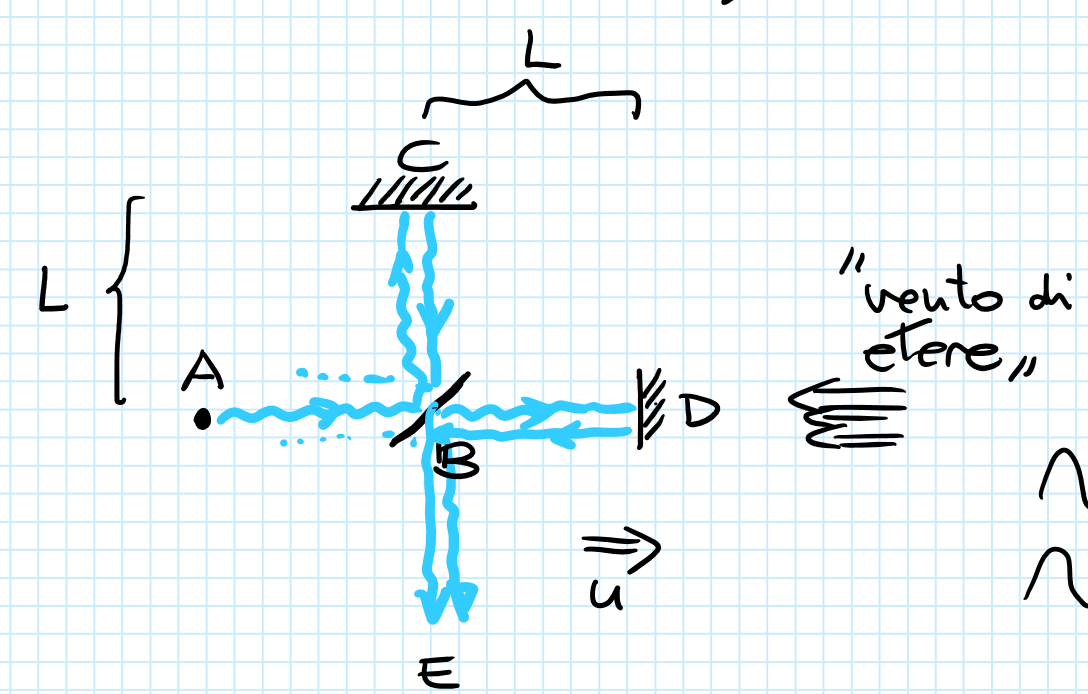
\includegraphics[width=7cm]{images/Vento_di_Etere.png}
\end{figure}
Supponiamo che il vento d'etere sia diretto lungo $BD$, cio\`e la terra si muove in quella direzione rispetto al riferimento dell'etere:
\begin{align*}
&t(BD)=t_1\\
&t(DB)=t_2\\
&t(BC)=t(CB)=t_3
\end{align*}
Se $L$ \`e la lunghezza di $BD$ e di $BC$, se $u$ \`e la velocit\`a dell'a terra rispetto all'etere allora
\[t_1=\frac L{c-u}\quad t_2=\frac L{c+u}.\]
Consideriamo ora il sistema di riferimento dove la velocit\`a della luce \`e $c$, cio\`e nel sistema solidale all'etere:\\
Per quanto riguarda il tratto $BD$ in questo sitema 
\[ct_1=L+ut_1,\quad ct_2=L-ut_2\quad\implies\quad t_1+t_2=\frac{2Lc}{c^2-u^2},\]
mentre sul tratto $BC$ si ha
\[(ct_3)^2=L^2+(ut_3)^2\quad\implies\quad t_3=\frac L{\sqrt{c^2-u^2}}\]
e il tempo che ci interessa \`e $2t_3$. Si ha dunque
\[2t_3=\frac{2L}{\sqrt{c^2-u^2}}\neq \frac{2Lc}{c^2-u^2}=t_1+t_2.\]
Ammettiamo allora di aver sbagliato qualche misura in modo tale che le distanze $BC$ e $BD$ non siano identiche. Si pu\`o ricavare
\[t_1+t_2-2t_3\approx \frac{2L_{BD}}c\pa{1+\frac{u^2}{c^2}}-\frac{2L_{BC}}c\pa{1+\frac{u^2}{2c^2}}.\]
Se ruotiamo l'esperimento, l'effetto \`e scambiare i valori di $L_{BD}$ e $L_{BC}$ ma in ogni caso non \`e stata misurata una differenza.
\end{proof}
\noindent
Cosa potrebbe star succedendo?
\setlength{\leftmargini}{0cm}
\begin{enumerate}
\item[$\boxed{Fizeau}$] Magari la terra trascina l'etere e la luce. Se $n$ \`e l'indice di rifrazione tra due mezzi (in questo caso etere ed etere trascinato), la luce va a velocit\`a $c$ nell'etere e ci stiamo muovendo a velocit\`a $u$ rispetto a questo, si ha che la velocit\`a della luce sarebbe
\[\frac cn+u\pa{1-\frac1{n^2}}.\]
\item[$\boxed{Fitzgerald}$] Magari le lunghezze parallele parallele alla direzione di modo si contraggono
\[L_{\parallel}=L_0\sqrt{1-\frac{u^2}{c^2}}.\]
Con questo cambiamento la differenza tra i tempi riscontrata nell'esperimento di Michelson-Morley effettivamente si annulla. 
\end{enumerate}
\setlength{\leftmargini}{0.5cm}
\noindent Resta ancora una questione: se osserviamo l'esperimento di Michelson-Morley in movimento, il tempo che la luce sembra impiegare per percorrere il tratto perpendicolare alla direzione del moto aumenta
\[\frac{2L}c \quad\text{ contro }\quad \frac{2L}c\frac1{\sqrt{1-\frac{u^2}{c^2}}}.\]
Questo sembra indicare che anche la coordinata temporale cambia cambiando sistema di riferimento. 

\section{Trasformazioni di Lorenz}
\begin{definition}[Frazione della velocit\`a della luce]
Data una velocit\`a $u$, essa corrisponde alla \textbf{frazione della velocit\`a della luce} data da
\[\beta(u)=\frac{u}c.\]
Se $u$ \`e chiara da contesto scriviamo solo $\beta$.
\end{definition}
\begin{definition}[Fattore di Lorenz]
Definiamo il \textbf{fattore di Lorenz} relativo alla velocit\`a $u$ come
\[\gamma(u)=\frac1{\sqrt{1-\frac{u^2}{c^2}}}=\frac1{\sqrt{1-\beta(u)^2}}.\]
Quando $u$ \`e chiara dal contesto scriviamo solo $\gamma$.
\end{definition}
\begin{remark}
$\gamma(u)$ \`e sempre maggiore o uguale a $1$ in quanto $0\leq u\leq c$.
\end{remark}

\begin{remark}
La correzione di Fitzgerald corrisponde a dire $\gamma L_\parallel=L_0$. 
\end{remark}
\noindent Dato che la correzione di Fitzgerald sulle lunghezze funziona, deduciamo per il principio di relativit\`a che
\[x=\frac{x'}\gamma+ut,\qquad x'=\frac{x}\gamma-ut',\]
da cui ricaviamo le \textbf{trasformazioni di Lorenz}
\[\begin{cases}
t'=\gamma\pa{t-\frac{ux}{c^2}}\\
x'=\gamma (x-ut)\\
y'=y\\
z'=z
\end{cases}\]
\begin{remark}
Se $\beta\to 0$ allora $\gamma\to 1$ e quindi ritroviamo le trasformazioni di Galileo.
\end{remark}
\noindent
Possiamo scrivere le trasformazioni di Lorenz in modo equivalente nella forma
\[\begin{cases}
ct'=\gamma\pa{ct-\beta x}\\
x'=\gamma (x-\beta ct)\\
y'=y\\
z'=z
\end{cases}\coimplies\mat{ct'\\x'\\y'\\z'}=\mat{\gamma & -\beta\gamma &&\\ -\beta\gamma & \gamma &&\\&&1&\\&&&1}\mat{ct\\x\\y\\z}\]
\noindent Osserviamo che
\[\begin{cases}
\pp t{}=\pp {t}{t'}\pp{t'}{}+\pp t{x'}\pp {x'}{}+\pp t{y'}\pp {y'}{}+\pp t{z'}\pp {z'}{}=\gamma\pp{t'}{}-\gamma u\pp{x'}{}\\
\pp x{}=\pp {x}{t'}\pp{t'}{}+\pp x{x'}\pp {x'}{}+\pp x{y'}\pp {y'}{}+\pp x{z'}\pp {z'}{}=-\gamma \frac{u}{c^2}\pp{t'}{}+\gamma \pp{x'}{}\\
\pp y{}=\pp {y}{t'}\pp{t'}{}+\pp y{x'}\pp {x'}{}+\pp y{y'}\pp {y'}{}+\pp y{z'}\pp {z'}{}=\pp {y'}{}\\
\pp z{}=\pp {z}{t'}\pp{t'}{}+\pp z{x'}\pp {x'}{}+\pp z{y'}\pp {y'}{}+\pp z{z'}\pp {z'}{}=\pp {z'}{}
\end{cases}\]

\begin{proposition}[Trasformazioni di Lorenz per direzioni arbitrarie]\label{LorenzDirezioneArbitraria}
Per un moto rettilineo uniforme a velocit\`a $\vec u$ si ha
\[\begin{cases}
\vec x'=\vec x+(\gamma -1)\frac{\vec x\cdot \vec u}{u^2}\vec u-\gamma t \vec u\\
t'=\gamma\pa{t-\frac{\vec u\cdot \vec x}{c^2}}
\end{cases}\]
\end{proposition}
\begin{proof}
Basta notare che la componente parallela al moto \`e
\[\vec x_\parallel=\frac{\vec x\cdot \vec u}{u}\frac{\vec u}{u}\]
mentre quella perpendicolare \`e $\vec x_\perp=\vec x-\vec x_\parallel$.
\end{proof}


\begin{definition}[Intervallo invariante]
L'\textbf{intervallo invariante} \`e
\[(ct)^2-x^2-y^2-z^2.\]
\end{definition}
\begin{proposition}
L'intervallo invariante \`e invariante per trasformazioni di Lorenz.
\end{proposition}
\begin{proof}
A meno di ruotare gli assi supponiamo che il moto avvenga lungo l'asse del moto relativo tra i sistemi (che supponiamo essere l'asse $x$). La tesi segue dal seguente calcolo
\begin{align*}
(ct')^2-(x')^2-(y')^2-(z')^2=&\gamma^2(ct)^2+\gamma^2\beta^2x^2-2\gamma^2 utx+\\
&-\gamma^2x^2-\gamma^2\beta^2(ct)^2+2\gamma^2 u tx-y^2-z^2=\\
=&\gamma^2(1-\beta^2)(ct)^2+\gamma^2(\beta^2-1)x^2-y^2-z^2=\\
=&(ct)^2-x^2-y^2-z^2.
\end{align*}
\end{proof}

\begin{remark}
Se stiamo misurando della luce allora l'intervallo invariante vale $0$.
\end{remark}

\begin{example}[Equazione delle onde]
Consideriamo l'equazione
\[\nabla^2\phi=\frac1{c^2}\pps[2]t\phi.\]
Si ha che questa equazione \`e invariante per le trasformazioni di Lorenz.
\end{example}
\begin{proof}
Segue sfruttando quanto sappiamo sui differenziali per le trasformazioni di Lorenz:
\begin{align*}
-\frac1{c^2}\pps[2]t\phi+\pps[2]x\phi+\pps[2]y\phi+\pps[2]z\phi=&-\frac1{c^2}\pa{\gamma^2\pps[2]{t'}{}-2\gamma^2 u\pp[2]{t'\del x'}{}+\gamma^2u^2\pps[2]{x'}{}}\phi+\\
&+\pa{\gamma^2\frac{u^2}{c^4}\pps[2]{t'}{}-2\gamma^2\frac{u}{c^2}\pp{t'\del x'}{^2}+\gamma^2\pps[2]{x'}{}}\phi+\\
&+\pps[2]{y'}\phi+\pps[2]{z'}\phi=\\
=&-\frac1{c^2}\pps[2]{t'}\phi+\pps[2]{x'}\phi+\pps[2]{y'}\phi+\pps[2]{z'}\phi.
\end{align*}
\end{proof}


\subsection{Dilatazione dei tempi e contrazione delle lunghezze}
\begin{definition}[Intervallo di tempo proprio]
Consideriamo due eventi che nel sistema di riferimento $S'$ hanno la stessa posizione. L'intervallo di tempo misurato da un orologio fermo rispetto a $S'$ tra questi \`e detto \textbf{intervallo di tempo proprio} tra i due
\[\Delta t'=\Delta t_0\]
\end{definition}

\noindent
Sia $\Delta t'=t_1'-t_2'$ l'intervallo di tempo proprio tra due eventi. Cambiando sistema di riferimento troviamo
\[\Delta t=t_1-t_2=\frac{\Delta t'+\cancelto0{\Delta x'} \frac{u}{c^2}}{\sqrt{1-\frac {u^2}{c^2}}}=\gamma \Delta t'\]
dunque l'intervallo di tempo misurato da un sistema in movimento rispetto alla posizione dei due eventi \`e maggiore rispetto a quello misurato da un sistema che li vede alla stessa posizione.\\
Questo fenomeno \`e detto \textbf{dilatazione dei tempi}.
\bigskip


\begin{definition}[Lunghezza propria]
Fissiamo un sistema di riferimento $S'$ e consideriamo una distanza $\Delta x'$ tra due punti fermi in questo sistema. Questa \`e detta la \textbf{lunghezza propria}.
\end{definition}
Sia $\Delta x'$ la distanza misurata tra due punti fermi rispetto a $S'$ in $S'$. Cambiando sistema di riferimento troviamo
\[\Delta x=x_1-x_2=\frac{\Delta x'+u\Delta t'}{\sqrt{1-\frac{u^2}{c^2}}}\]
Affinch\'e la misura di questa lunghezza abbia senso in $S$ dovremo avere $\Delta t=0$ (mentre $\Delta t'$ a priori pu\`o essere qualsiasi valore, tanto la distanza in $S'$ non dipende dal tempo). Consideriamo dunque la trasformazione inversa
\[\Delta x'=\frac{\Delta x-u\cancelto0{\Delta t}}{\sqrt{1-\frac{u^2}{c^2}}}=\gamma \Delta x\]
dunque $\Delta x=\gamma\ii \Delta x'$, cio\`e la lunghezza misurata in $S$ \`e pi\`u piccola rispetto a quella in $S'$.\\
Questo fenomeno \`e detto \textbf{contrazione delle lunghezze}.

\begin{example}[Relativit\`a della simultaneit\`a]
Se due osservatori sono in moto l'uno rispetto all'altro e uno dei due misura due eventi con posizioni diverse ma allo stesso istante allora il secondo osservatore vede i due eventi come non simultanei. Questo segue immediatamente da
\[\Delta t'=\gamma\pa{\Delta t-\frac{u\Delta x}{c^2}}=-\frac{\gamma u}{c^2} \Delta x\neq 0.\]
\end{example}



\section{Trasformazioni di velocit\`a}
\begin{proposition}[Formula di Boost]\label{FormulaBoost}
Se un oggetto si muove parrallelo al moto tra due sistemi di riferimento inerziali allora
\[v'=\dfrac{v-u}{\displaystyle 1-\frac{uv}{c^2}}=\pa{\frac{\beta(v)-\beta(u)}{1-\beta(v)\beta(u)}}c.\]
\end{proposition}
\begin{proof}
Consideriamo $x(t)=vt$ e portiamo nel sistema $S'$
\[x'=\gamma(x-ut)=\gamma(v-u)t=\gamma^2(v-u)\pa{t'+\frac{ux'}{c^2}}\]
dunque
\[x'\pa{1-\frac u{c^2}\gamma^2(v-u)}=\gamma^2(v-u)t',\]
da cui 
\[x'=\frac{v-u}{1-\frac{u^2}{c^2}-\frac u{c^2}(v-u)}t'=\frac{v-u}{1-\frac{uv}{c^2}}t'.\]
\end{proof}

\begin{remark}
Considerando i limiti $\beta(u)\to 0$ e $\beta(v')\to 0$ allora ritroviamo il Boost Galileiano.
\end{remark}

\begin{remark}
Se $v=c$ oppure $u=c$ troviamo $v'=c$, che \`e l'assioma sulla costanza della velocit\`a della luce.
\end{remark}

\begin{remark}
Se il moto non \`e allineato con quello dei sistemi troviamo
\[\begin{cases}
\displaystyle v_x'=\frac{v_x-u}{1-\frac{v_x u}{c^2}}=\frac{v_x-u}{1-\beta(v_x)\beta(u)}\\\\
\displaystyle v_y'=\dfrac{v_y}{\gamma(u)\pa{1-\frac{v_x u}{c^2}}}=\frac{v_y}{\gamma(u)\pa{1-\beta(v_x)\beta(u)}}\\\\
\displaystyle v_z'=\dfrac{v_z}{\gamma(u)\pa{1-\frac{v_x u}{c^2}}}=\frac{v_z}{\gamma(u)\pa{1-\beta(v_x)\beta(u)}}
\end{cases}\]
\end{remark}

\noindent La formula vettoriale per il boost di Lorenz \`e
\[\vec v'=\frac1{1-\frac{\vec u\cdot \vec v}{c^2}}\pa{\frac1\gamma \vec v-\vec u+\pa{1-\frac1\gamma}\frac{\vec u\cdot \vec v}{u^2}\vec u}\]
o equivalentemente
\[\vec v'=\frac1{1-\frac{\vec u\cdot \vec v}{c^2}}\pa{\vec v-\vec u+\pa{1-\frac1\gamma} \frac{\vec u\times (\vec u\times \vec v)}{u^2}}\]


\begin{example}[Formula di Fizeau]
Consideriamo come cambia la velocit\`a della luce entro un mezzo con indice di rifrazione $n$ tra due sistemi in moto relativo a velocit\`a $u$:
\[v=\frac{c/n+u}{1+\frac{cu}{nc^2}},\]
da cui la differenza tra le velocit\`a \`e
\[\Delta v=v-\frac cn=\frac{u(1-n^{-2})}{1+\frac{uc}{nc^2}},\]
che per $u\ll c$ si approssima a $u\pa{1-\frac1{n^2}}$.
\end{example}

